\documentclass{beamer}

\usepackage[utf8]{inputenc}
\usepackage{listings}

\usetheme{Warsaw}

\useoutertheme{infolines}
\setbeamertemplate{blocks}[default]
%% \setbeamertemplate{items}[circle]

% \logo{\includegraphics[width=15px,height=15px]{/home/wulczer/flumotion.png}}

\AtBeginSubsection[]
{
  \begin{frame}{Outline}
    \tableofcontents[sectionstyle=show/shaded,subsectionstyle=show/shaded/hide]
  \end{frame}
}

\title{Replacing GEQO}
\subtitle{Join ordering via Simulated Annealing}
\author{Jan Urbanski \\ \texttt{j.urbanski@wulczer.org}}
\institute{University of Warsaw / Flumotion}
\date{\today}

\begin{document}

\lstset{language=C}

\frame{\titlepage}

\begin{frame}
  \tableofcontents
\end{frame}

\section{The problem}
\subsection{Determining join order for large queries}

\begin{frame}
  \frametitle{Getting the optimal join order}

  \begin{itemize}
  \item part of of planning a query is determining the order in which relations
    are joined
  \item it is not unusual to have queries that join lots of relations
  \item JOIN and subquery flattening contributes to the number or relations to
    join
  \item automatically generated queries can involve very large joins
  \end{itemize}
\end{frame}

\begin{frame}
  \frametitle{Problems with join ordering}

  \begin{itemize}
  \item finding the optimal join order is an NP-hard problem
  \item considering all possible ways to do a join can exhaust available memory
  \item not all join orders are valid, because of:
    \begin{itemize}
    \item outer joins enforcing a certain join order
    \item IN and EXISTS clauses that get converted to joins
    \end{itemize}
  \item joins with restriction clauses are preferable to Cartesian joins
  \end{itemize}
\end{frame}

\subsection{GEQO, the genetic query optimiser}

\begin{frame}
  \frametitle{Randomisation helps}

  \begin{itemize}
  \item PostgreSQL switches from exhaustive search to a randomised algorithm
    after a certain limit
  \item GEQO starts by joining the relations in any order
  \item and then proceeds to randomly change the join order
  \item genetic algorithm techniques are used to choose the cheapest join order
  \end{itemize}
\end{frame}

\begin{frame}
  \frametitle{Problems with GEQO}

  \begin{itemize}
  \item has lots of dead/experimental code
  \item there is a TODO item to remove it
  \item nobody really cares about it
  \item is an adaptation of an algorithm to solve TSP, not necessarily best
    suited to join ordering
  \item requires some cooperation from the planeer, which violates abstractions
  \end{itemize}
\end{frame}

\section{The solution}

\subsection{Simulated Annealing overview}

\begin{frame}
  \frametitle{What is Simulated Annealing}

  \begin{columns}
    \begin{column}{7cm}
      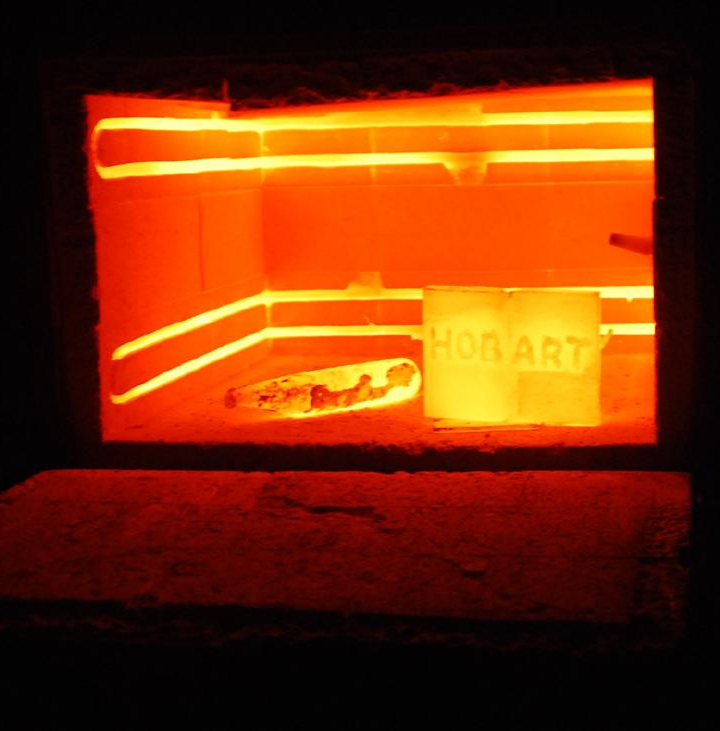
\includegraphics[width=7cm]{furnace.png}
    \end{column}
    \begin{column}{5cm}
      Annealing (...) is a process that produces conditions by heating to above
      the re-crystallization temperature and maintaining a suitable
      temperature, and then cooling.\\
      \hfill\textit{-- Wikipedia}
    \end{column}
  \end{columns}
\end{frame}

\begin{frame}
  \frametitle{The SA Algorithm - cont.}

  \begin{itemize}
  \item the system starts with an initial temperature and a random state
  \item uphill moves are accepted with probability that depends on the current
    temperature
    \begin{block}{probability of accepting an uphill move}
      \begin{equation*}
        p = e^{\frac{cost_{prev} - cost_{new}}{temperature}}
      \end{equation*}
    \end{block}
  \item moves are made until equilibrium is reached
  \item temperature is gradually lowered
  \item once the system is frozen, the algorithm ends
  \end{itemize}

\end{frame}

\begin{frame}[fragile]
  \frametitle{The SA algorithm}

\begin{block}{Simulated Annealing}
\begin{semiverbatim}
\uncover<2->{state = \alert<7->{random\_state()}}
\uncover<6->{do \{}
\uncover<4->{    do \{}
\uncover<3->{      new\_state = \alert<8->{random\_move()}}
\uncover<3->{      if (\alert<9->{acceptable(}new\_state\alert<9->{)})}
\uncover<3->{        state = new\_state}
\uncover<4->{    \}}
\uncover<4->{    while (!\alert<10->{equilibrium()})}
\uncover<5->{    \alert<11->{reduce\_temperature()}}
\uncover<6->{\}}
\uncover<6->{while (!\alert<12->{frozen()})}
\uncover<6->{return state}
\end{semiverbatim}
\end{block}

\end{frame}

\begin{frame}
  \frametitle{The SA Algorithm - cont.}

Implementing Simulated Annealing means solving the following problems:

  \begin{itemize}
  \item finding an initial state
  \item generating subsequent states
  \item defining an acceptance function
  \item determining the equilibrium condition
  \item suitably lowering the temperature
  \item determining the freeze conditions
  \end{itemize}
\end{frame}

\begin{frame}
  \frametitle{A visual example}
  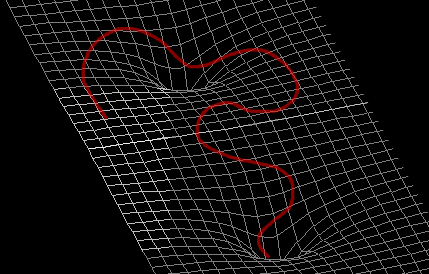
\includegraphics[width=\textwidth]{curve.png}
\end{frame}

\subsection{PostgreSQL specifics}
\subsection{Query tree transformations}

\section{The results}
\subsection{Comparison with GEQO}

\section{The future}
\subsection{Development focuses}


\section{The end}
\subsection{Questions}


\begin{frame}
\end{frame}

\end{document}
